\section{Stability}
Determining the stability in a system is important for a number of applications. How do we ascertain a system will not react uncontrollably to some input? Will a certain system come to an equilibrium or rapidly diverge? 

We have a pretty good intuition for what stability is, but to give a more formal definition: a system is said to be stable if for some bounded input, also the output will remain bounded. Technically, by this definition, a system may act unstable given an impulse input ($\delta(t)$) since this signal isn't bounded, but in practise this does not pose a problem because we can't produce unbounded signals in reality.

There are several methods for determining system stability, which are all useful in different cases. These methods include Bode plots, the root locus method, the Routh-Hurwitz criterion, and the Nyquist criterion. In the next section we will study this last method in detail.

\subsection{The Nyquist Criterion of Stability}
The Nyquist criterion uses the location of zeroes and poles in the transfer function of a system in order to determine stability. In order to locate these poles and zeroes, ``Cauchy's argument principle'' is used. As this is key to understand the Nyquist criterion, we will take a closer look at what it states in a little bit.
%To explain the Nyquist criterion we must start with Cauchy's argument principle. This principle is used to find the difference between the number of poles and zeroes inside some closed contour.

The Nyquist criterion states that if all poles in a system's transfer function lies in the negative half of the complex number plane (i.e. real part of $z<0$), the system is stable. Let's take a look at why this is the case.

As shown in section \ref{sec:combsys}, a control system can always be expressed as a fraction of two transfer functions. \todo{Write somewhere about OL and CL, I think}The question about poles of a system's transfer function can therefore be rephrased as a question about zeroes in the transfer function in the denominator.

Let's first define a transfer function by its poles and zeroes in the following way:
\begin{code}
--                             zeros poles
data TransferFunc = TransferFunc [C] [C]
\end{code}
\begin{equation*}
    \text{TransferFunc}([z_0,z_1,...]; [p_0,p_1,...])=\frac{(s-z_0)(s-z_1)...}{(s-p_0)(s-p_1)...}
\end{equation*}
\LNContinue
As the poles do not change when multiplying the function by some bounded function (we assume the fraction is fully reduced, i.e. nothing like (s-1)(s-2)/(s-1)), \cmd{TransferFunc a b} is equivalent to \cmd{TransferFunc [] b} in terms of where poles are. Recall the fact that a fraction of the form $\frac{1}{ab}$ can be written $\frac{A}{a}+\frac{B}{b}$. %Also notice how \cmd{a * TransferFunc c d} has the same poles and zeroes as \cmd{TransferFunc c d}.
In the following pseudocode, let \cmd{f ~== g} denote that functions f and g have the same poles (not zeroes), and \cmd{TF} be short for \cmd{TransferFunc}.
\begin{codeeq}
TF a b ~== TF [] b
TF [] [b0,b1,...] ~== TF [] [b0] + TF [] [b1] + ... ==
  == laplace $ \t -> exp (t*b0) + exp (t*b1)+...
\end{codeeq}
%(Refer to appendix \ref{sec:applap} for $\mathcal{L}^{-1}$)\\

Notice how \cmd{\t -> exp (t*bx)} would be exponential decay if \cmd{bx} is negative. This is to say that when \cmd{t} is large, the signal tends to 0. Crucially, this is \textit{only} true when bx (denoting b0, b1, etc.) is negative. If bx would be positive, then the function would be exponentially increasing instead, which would be an unstable system. (If bx would be 0, then the function would be constant 1). Since b are the poles of \cmd{TransferFunc [] b}, we see that system stability is equivalent to whether the poles of the system's transfer function lies in the negative half of the complex plane. To understand how to determine this, we should take a look at Chauchy's arguement principle.
\missingfigure[]{Figure showing exponential decay (if useful and not already included in \ref{sec:decay})}



This theorem uses a the notion of a contour to relate movement around poles and zeroes and movement around the origin, so we must first be clear about what a contour is: 

\subsubsection{Contours}

Think of a contour as all of the values along a closed loop in the complex plane (in generality not limited to the complex plane; a contour may be on any (multidimensional) ``sheet''). For example, consider the unit circle in the complex plane, centered at the origin. We might mathematically describe this contour by the set of points' unit distance from the origin: $\left\{z\in\mathbb{C} : |z|=1\right\}$. 
\missingfigure[]{unit circle contour?}
Since $\mathbb{C}$ is not only infinite in size, but \textit{uncountably} infinite (meaning elements cannot be listed, even with infinite terms/time), we cannot accurately represent this in Haskell---even with infinite lists. What we can do, though, is approximate it in Haskell (with finite or infinite lists). In the code below, \cmd{cos} and \cmd{sin} are used to trace out the unit circle, and \cmd{d} specifies the distance between consecutive points. When $d\rightarrow0^+$ \cmd{ucContour} tends to \textit{an approximation} of the unit circle contour.
\begin{code}
ucContour :: R -> [C]
ucContour d = [C (cos (2*pi*k//n)) (sin (2*pi*k//n)) | k<-[0..n]] where
  n = floor (2*pi/d)
  a // b = fromIntegral a / fromIntegral b
\end{code}
Let's now define a more general function for contours, that will take a list of points and then subdivide this into an approximated contour of specified accuracy. We start with defining \cmd{subdiv} as a function that subdivides one such line segment (defined by two complex numbers):\todo{Use complex number defined in material!}
\begin{code}
(*&) :: R -> C -> C
c *& C r i = C (c * r) (c * i)
infixl 7 *& -- same as *

subdiv :: R -> (C, C) -> [C]
subdiv d (a, b) = [ a + n *& seg | n <- [1..nseg]] where
  len = re.abs $ b - a
  nseg = fromIntegral.floor $ len / d
  seg = (d / len) *& (b - a)
\end{code}
Now, we use this helper function to define \cmd{contourAng}. This function will subdivide a polygon described by a given list of vertices, into a more numerous list of points, to specified accuracy.
\begin{code}

contourAng :: R -> [C] -> [C]
contourAng dist points = concatMap (subdiv dist) $ pairs ps where
  ps = points ++ [head points]
  pairs (a:b:cs) = (a,b) : pairs (b:cs)
  pairs [_]      = []
\end{code}

\missingfigure[]{This \textit{could} be illustrated by an image of a polygonal contour}
We can use this function in order to create polygonal contours in the complex plane. \todo[inline,noinlinepar,inlinewidth=3cm]{Introduce semicircle contour either here, or in "5.1.3 Nyquist Criterion"}

\subsubsection{Cauchy's Argument Principle}
%\todo[inline]{Cauchy and contour mapping (see code on github in play/tommy) (this will probably be lengthy)}
Cauchy's argument principle states that, given a transfer function F(s) (in code denoted \cmd{f}) and a contour C (in code denoted \cmd{c}) (with counter-clockwise direction), if F has z zeroes and p poles inside C, then the contour \cmd{map f c} will travel around the origin (z-p) times in the counterclockwise direction. 

\begin{figure}[h!]
    \centering
    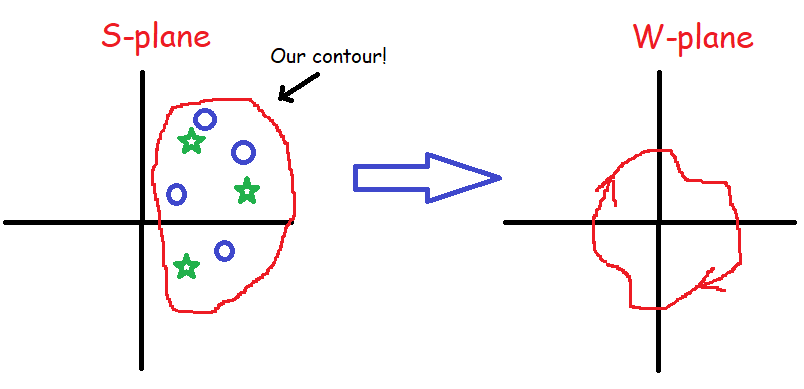
\includegraphics[scale= 0.4]{Images/sw.PNG}
    \caption{Mapping the values in a contour surrounding three zeroes and four poles in the s-plane (for a transfer function) is mapped to a contour surrounding the origin once. (This mapping is sometimes said to be in the ``W-plane.'')}
    \label{Cauchy}
\end{figure}

To show why this is the case, %let's take a look at a minimal case where we have one zero (at z0, and no poles) within a contour c for a transfer function F(s). For simplicity, assume F is a rational function (i.e. a fraction of polynomials) and in particular F(s)$=s-z0$. By definition F(z0)=0
consider the minimal case where we have a transfer function F(s)=(s-z0), which has a zero at z0. If we map F onto a contour C surrounding z0 in the complex plane, this is naturally equivalent to translating C with -z0. Since C is defined to surround z0, the translated contour will surround z0+(-z0)=0 (i.e. the origin). 
If we add a zero to the function (F$_2$(s)=(s-z0)(s-z1)) and let C surround both of these, \cmd{map f c} will be the element-wise product of the contours translated by -z0 and -z1, respectively. We can imagine how this will still encircle the origin, but, in fact, it will do so twice. This is because (as reminded in section \ref{sec:complex}) when multiplying two complex numbers, their arguments add---if both contours surrounds the origin once, their element-wise product should do so twice.
If, instead C surrounds only z0, when mapping (s-z1) on C, this translates C to surround (z0-z1) strictly without surrounding the origin.

In the general case, let F$_3$(s)=(s-z0)g(s), with a zero at z0, for some function g. In this case, the contour is translated separately by -z0 as well as the roots of g(s), and multiplied in the same way as before.
\missingfigure[]{Figure illustrating the translation could be in order}

All in all thus far, if C surrounds z zeroes of F, \cmd{map f c} will envelop the origin z times in the counter-clockwise direction.

The same argument could be made about the poles of a transfer function F(s). Let F(s)=Z(s)/P(s), where Z contains the zeroes of F, and P the poles of F as zeroes. The previous argument goes for Z(s), as well as the zeroes of P. When P is reciprocated, each point in \cmd{map p c} is reciprocated, and is as a consequence flipped over the real line\footnote{$1/(a+bi)=(a-bi)/((a+bi)(a-bi))=(a-bi)/(a^2-b^2)=(a-bi)c$. When reciprocated, $z=(a+bi)$ is conjugated (flipped over real line) and scaled by $c=a^2-b^2$}. This flips the direction of C from counter-clockwise to clockwise. 

From these two arguments, we see that F mapped over a contour C which encircles z zeroes and p poles of F once in the counter-clockwise direction, will encircle the origin (z-p) times. This is what Cauchy's argument principle states.

%According Cauchy's we start by mapping each value on our contour to our function and create a new plot (works exactly the same as Haskell's map). This new plot will, among other properties, show us the difference between poles and zeroes. Depending on how many times the plot surround the origin, and in which direction, we can get information about the poles and zeroes. Let me show you with a picture.


%Inside our contour we got four zeroes and tree poles. After we map all the values in the contour the plot in the w-plane is created. The plot surrounds the origin one time clockwise. This tells us that we got one more zero than pole inside our contour. If the plot was counterclockwise we would have had more poles than zeroes instead.

\subsubsection{Nyquist Criterion}
\todo[inline]{Tie together with N=Z-P}
As mentioned earlier, the Nyquist criterion states that if there are no poles in the positive side of the complex plane of a transfer function F, its corresponding system is stable. If we assume we have the function P in F(s)=Z(s)/P(s), where Z contains all zeroes of F and P all poles of F as zeroes, we can check whether P has any zeroes in the positive side of the complex plane using Cauchy's argument principle. We do this by placing a contour that surrounds all of the positive side of the complex plane. By mapping P onto this contour, we get the number of zeroes minus the number of poles in this half-plane, as the so-called winding-number (the number of times the contour travels around the origin in the counter-clockwise direction). Assuming we know P to have no poles (in the positive side of the complex plane), we can use this principle directly: if the mapped contour encircles the origin, the system is unstable; if it does not, it is stable.

\begin{figure}[h!]
    \centering
    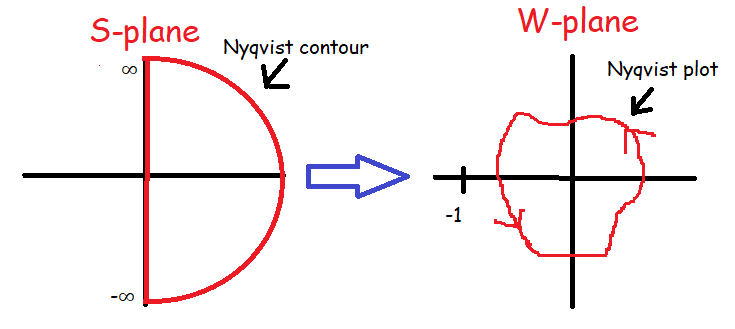
\includegraphics[scale= 0.4]{Images/nykv.PNG}
    \caption{Placing a contour that surrounds all of the right-hand side of the complex plane, and mapping with a (transfer) function gives us the so-called Nyquist plot. If this surrounds the origin, the system the transfer function describes is stable.}
    \label{Nyqvist}
\end{figure}\todo{Place image appropriately}

Since stability is only relevant for closed-loop systems (and therefore contain a feedback loop), P will have the form P(s)$=1-\text{G}(s)=1-\smashoperator{\sumprod_{x}}{(s-\text{px})}$, as seen in section \ref{sec:combsys}. Therefore, the Nyquist criterion is often stated in terms of the transfer function G, where the mapped contour instead would wind around (-1) instead of the origin.

The criterion can be simplified somewhat by changing the contour to a non-closed contour going from \cmd{C 0 (-Infinity)} to \cmd{C 0 (Infinity)} and looking only at whether \cmd{map g c} passes above or below (-1) on its way to the origin. This only works for negative feedback-loops, however. This is often called the simplified Nyquist criterion. %\todo[inline,noinlinepar,inlinewidth=1cm]{wip}\todo[inline,noinlinepar,inlinewidth=3cm]{simplified NC}


%Nyquist theorem will use this principle to find out if a system i stable or not. The Nyquist theorem is graphical technique and will result in a Nyquist plot. In the case of the a closed loop system the transfer function is defined as

%\begin{equation*}
%F(s) \ (1 + F(s)H(s))
%\end{equation*}

%That means if our denominator is equal to zero our system is unstable. That would be bad news!

%To solve this we want to find out if we got any zeros in our right half plane. Therefore we surround our entire right half plane with a contour with infinite radius. We could map all these values to our denominator 
%\begin{equation*}
%1 + F(s)H(s)
%\end{equation*}

%but instead we are going to map our values to \begin{equation*}
%F(s)H(s)
%\end{equation*}

%to make our lives easier. The will result of this will is the Nyquist plot. Since we removed our +1 we a going to count the encirclements around -1 instead of the origin. In the picture you can take a look at this.



%Unfortunately this will only give us the difference between the number of zeroes and poles. To solve this will will utilise the equation $Z = N + P$. Where Z is the number of zeroes, N the number of clock wise encirclements and P is the number of poles in the open loop. In other words Nyquist let us solve the closed-loop system with some help from the open-loop system.


%This is how a Nyquist plot is created and what i tell us about a transfer function. But since neither we or Haskell's map function can't compute with a infinite large input we have to find a way around this. We can instead focus on four important points and get a non-continuous plot. w=0, w=inf, w when we cross the real axis and w when we cross the imaginary axis. This will be enough for the most basic transfer functions you will see in the course.

